%%%%%%%%%%%%%%%%%%%%%%%%%%%%%%%%%%%%%%%%%%%%%%%%%%%%%%%%%%%
% Technical report written with the Tau-class template
% (Guillermo Jimenez, CC BY 4.0, https://github.com/MemoJimenez/Tau-class).
% Compile: pdflatex -> biber -> pdflatex -> pdflatex
%%%%%%%%%%%%%%%%%%%%%%%%%%%%%%%%%%%%%%%%%%%%%%%%%%%%%%%%%%%

\documentclass[9pt,a4paper,twocolumn,twoside]{tau-class/tau}
\usepackage[english]{babel}
\graphicspath{{../../src/figures/}}
\raggedbottom % do not stretch a column to match the other one
\setlength{\eqskip}{16pt} % space around display equations (template default 9pt is too tight)

% Source files are read directly, so the listings always match the code.
\newcommand{\src}[1]{../../src/tsn_gate/#1}
% amsmath is not loaded (stix2 must come after it), so define the few helpers used here.
\providecommand{\eqref}[1]{(\ref{#1})}
\providecommand{\secref}[1]{Section~\ref{#1}}
\lstset{language=Python, basicstyle=\scriptsize\ttfamily, tabsize=4, numbers=left, numbersep=4pt,
  numberstyle=\tiny\color{taucodecomment}, xleftmargin=1.4em,
  postbreak=\mbox{\scriptsize\textcolor{taucodecomment}{$\hookrightarrow$}\space}}

%----------------------------------------------------------
% Title & Authors/Affiliations
%----------------------------------------------------------

\doctype{Technical Report}
\title{A Certified Admission Gate for TSN: From Network-Calculus Equations to Code}

\author[a]{Huyen-Trang Le\thanks{\href{mailto:huyen.le@etud.univ-evry.fr}{huyen.le@etud.univ-evry.fr} (H.-T. Le), \href{mailto:aakash.soni@ece.fr}{aakash.soni@ece.fr} (A. Soni), \href{mailto:samia.bouzefrane@lecnam.net}{samia.bouzefrane@lecnam.net} (S. Bouzefrane)}}
\author[b]{Aakash Soni}
\author[c]{Samia Bouzefrane}

\affil[a]{IBISC Laboratory, Universit\'e d'\'Evry Paris-Saclay, \'Evry-Courcouronnes, France}
\affil[b]{LyRIDS Laboratory, ECE Paris, Paris, France}
\affil[c]{CEDRIC Laboratory, Conservatoire National des Arts et M\'etiers (Cnam), Paris, France}

\dates{This report was compiled on \today}
\docinfo{Companion to the four-page note \textit{A Certified Admission Gate for Online Reconfiguration of Time-Sensitive Networks}. Source code: \url{https://github.com/hazel260802/network-calculus}.}

\footinfo{Certified TSN admission gate}
\leadauthor{H.-T. Le et al.}

%----------------------------------------------------------
% Abstract and Keywords
%----------------------------------------------------------

\begin{abstract}
This technical report documents how the problem of online admission control in Time-Sensitive Networking (TSN) is formulated and how its solution is structured in code. The problem is the following: in a running TSN with a set of admitted flows, decide for each new flow request whether it can be added without any admitted flow missing its worst-case deadline, and prove the decision. We formulate it on a model of 1\,Gbit/s switches with fixed shortest-path (ECMP) routing, token-bucket flows and non-preemptive static-priority ports, and solve it with deterministic network calculus: a per-hop delay bound derived from the residual service of each priority class, burst propagation along each path, and Total Flow Analysis for the end-to-end bound. For each equation, the report shows the function and lines of the Python package \texttt{tsn\_gate} that compute it. It then explains how the implementation is organised: the full and incremental admission gates, the certificate and its seven checking conditions, the packet-level simulator and the cross-check against the reference tool panco, with a two-flow example worked by hand. Every number produced by the code can thus be re-derived on paper.
\end{abstract}

\keywords{Time-Sensitive Networking, deterministic network calculus, admission control, static priority, certificates}

%----------------------------------------------------------

\begin{document}

    \maketitle
    \thispagestyle{firststyle}
    \tableofcontents

%----------------------------------------------------------

\section{Purpose and Structure of the Code}

    \taustart{T}SN provides bounded latency on switched Ethernet~\cite{ieee8021q,lobello2019tsn}, but its guarantees rest on an analysis of the whole flow set. When flows are added at run time, each addition can increase the delay of flows already admitted, including flows on other paths that share a port. The gate implemented here answers one question per request: \emph{after adding this flow, does every admitted flow still meet its deadline?} It answers with a verdict and with evidence, a certificate, that can be checked without trusting the analysis code.

    The implementation is the Python package \inlinecode{tsn_gate} in the public repository~\cite{tsnrepo}. \tabref{tab:modules} maps each module to the part of the mathematical model it implements; the rest of this report follows the same order.

    \begin{table}[H]
        \caption{Modules of \texttt{tsn\_gate} and the model they implement}
        \label{tab:modules}
        \begin{tabular}{
            >{\raggedright\arraybackslash}p{0.27\columnwidth}
            >{\raggedright\arraybackslash}p{0.43\columnwidth}
            >{\raggedright\arraybackslash}p{0.17\columnwidth}
        }
        \toprule
        \textbf{Module} & \textbf{Role} & \textbf{Equations} \\
        \midrule
        \inlinecode{model.py} & Flows, network, routing, feed-forward check & \eqref{eq:ports}--\eqref{eq:topo} \\
        \inlinecode{topologies.py} & Reference two-tier topologies & \eqref{eq:portcount} \\
        \inlinecode{workload.py} & Seeded flow requests & \eqref{eq:tb} \\
        \inlinecode{analysis.py} & Per-port bound, burst propagation, TFA & \eqref{eq:residual}--\eqref{eq:e2e} \\
        \inlinecode{gate.py} & Full and incremental gates & \eqref{eq:sched} \\
        \inlinecode{certificate.py} & Witnesses, digest, checker C0--C6 & \eqref{eq:digest}--\eqref{eq:ge} \\
        \inlinecode{simulator.py} & Packet-level sanity check & \eqref{eq:emit} \\
        \bottomrule
        \end{tabular}
        \tabletext{Validation code (\texttt{validation/panco\_check.py}) and experiments (\texttt{experiments/}) sit next to the package.}
    \end{table}

    \subsection{Units and Notation}

        All quantities are in SI base units: bits, seconds and bit/s. A byte is the constant \inlinecode{BYTE = 8}, and the link rate is \inlinecode{GBPS = 1e9}. \tabref{tab:notation} lists the symbols used throughout and their names in the code.

        \begin{table}[!htbp]
            \caption{Notation and corresponding code identifiers}
            \label{tab:notation}
            \begin{tabular}{
                >{\raggedright\arraybackslash}p{0.17\columnwidth}
                >{\raggedright\arraybackslash}p{0.47\columnwidth}
                >{\raggedright\arraybackslash}p{0.23\columnwidth}
            }
            \toprule
            \textbf{Symbol} & \textbf{Meaning} & \textbf{Code} \\
            \midrule
            $C$ & Link rate of every port & \inlinecode{net.C} \\
            $t_{proc}$ & Constant processing delay per hop & \inlinecode{net.t_proc} \\
            $b_f, r_f$ & Burst and rate of flow $f$ & \inlinecode{f.b}, \inlinecode{f.r} \\
            $L_f$ & Maximum frame size of $f$ & \inlinecode{f.L} \\
            $k_f$ & Priority class of $f$ (0 highest) & \inlinecode{f.prio} \\
            $D^{\max}_f$ & End-to-end deadline of $f$ & \inlinecode{f.deadline} \\
            $\mathcal{P}_f$ & Ordered ports on the route of $f$ & \inlinecode{net.route()} \\
            $b^{(i)}_f$ & Input burst of $f$ at its $i$-th hop & \inlinecode{bursts[f][i]} \\
            $B_H, R_H$ & Burst and rate sums of higher classes & \inlinecode{B_H}, \inlinecode{R_H} \\
            $B_k, R_k$ & Burst and rate sums of class $k$ & \inlinecode{B_k}, \inlinecode{R_k} \\
            $L_{lo}$ & Largest frame of a lower class & \inlinecode{L_lo} \\
            $d_k(p)$ & Delay bound of class $k$ at port $p$ & \inlinecode{ClassBound.delay} \\
            $D_f$ & End-to-end bound of $f$ & \inlinecode{e2e[f]} \\
            $\tau(p)$ & Topological index of port $p$ & \inlinecode{net.topo_index[p]} \\
            \bottomrule
            \end{tabular}
        \end{table}

%----------------------------------------------------------

\section{System Model}

    \subsection{Network and Ports}

        The network is an undirected graph whose vertices are switches and end stations and whose edges are full-duplex links of rate $C$. Each direction of a link is an output \emph{port}, served by the node that transmits on it. For a link set $\mathcal{E}$, the port set is
        \begin{equation}\label{eq:ports}
            \mathcal{P} = \{(u,v) : \{u,v\} \in \mathcal{E}\} \cup \{(v,u) : \{u,v\} \in \mathcal{E}\},
        \end{equation}
        which \inlinecode{Network.ports()} returns sorted. Every port, including the egress port of a source end station, adds the constant processing delay $t_{proc}$ to the bound of every frame it serves; the simulator applies the same convention (\secref{sec:sim}).

    \subsection{Routing}

        Routing is fixed: each source--destination pair $(s,t)$ always uses the same path, and end stations never forward. \inlinecode{Network.route()} first computes, by breadth-first search from $t$, the hop distance $\delta(v)$ of every node $v$ that can reach $t$ through switches only. The path is then built from $s$ by always moving to a neighbour one hop closer to $t$:
        \begin{equation}\label{eq:route}
            v_{j+1} = N_j\big[\, h(s,t) \bmod |N_j| \,\big], \quad
            N_j = \mathrm{sort}\{v \sim v_j : \delta(v) = \delta(v_j) - 1\},
        \end{equation}
        where $h(s,t)$ is the CRC32 checksum of the string \inlinecode{"s->t"}. When several next hops are equally short, as between the core switches of a two-tier network, the hash spreads the pairs over them like Equal-Cost Multi-Path (ECMP) routing, while keeping the route of a pair fixed and reproducible across runs. Routes are cached in \inlinecode{_routes}.

        \begin{code}
            \lstinputlisting[firstline=56, lastline=85]{\src{model.py}}
            \caption{Shortest-path routing with ECMP tie-breaking (\texttt{model.py}).}
            \label{lst:route}
        \end{code}

    \subsection{Feed-Forward Check}

        Total Flow Analysis (TFA) as implemented needs the ports to be visited in an order where every port comes after all ports that feed it. Because routing is fixed, every flow that will ever be admitted follows one of the $|\mathcal{S}|(|\mathcal{S}|-1)$ routes between end stations $\mathcal{S}$. The constructor therefore builds, once, the \emph{port dependency graph}
        \begin{equation}\label{eq:depgraph}
            G = (\mathcal{P}, E), \quad (p,q) \in E \iff p, q \mbox{ are consecutive on some route},
        \end{equation}
        and computes a topological order with Kahn's algorithm, breaking ties by port name so the order is deterministic. The result is the index
        \begin{equation}\label{eq:topo}
            \tau : \mathcal{P} \to \{0, \dots, |\mathcal{P}|-1\}, \qquad (p,q) \in E \Rightarrow \tau(p) < \tau(q).
        \end{equation}
        If $G$ has a cycle, no such order exists and the constructor raises an error: the network is not feed-forward. A ring of six switches, for example, is rejected, whereas the two-tier topologies below pass because every route crosses at most one core switch.

    \subsection{Reference Topologies}

        \inlinecode{topologies.py} builds two-tier topologies: $n_c$ core switches, $n_e$ edge switches each linked to every core switch, and $e$ end stations per edge switch. (In the code the function is \inlinecode{leaf_spine}, the data-centre name of this structure.) The number of ports is twice the number of links:
        \begin{equation}\label{eq:portcount}
            |\mathcal{P}| = 2\,(n_c n_e + n_e e).
        \end{equation}
        The experiments use $(n_c, n_e, e) = (2, 4, 5)$, giving $2(8 + 20) = 56$ ports, and $(4, 8, 5)$, giving $2(32 + 40) = 144$ ports. A one-switch network with three end stations, \inlinecode{single_switch(3)}, is used for the hand-computed example of \secref{sec:example}.

    \subsection{Flows}

        A flow $f$ is a frozen data class \inlinecode{Flow(id, src, dst, b, r, L, prio, deadline)}. At its source it is constrained by the token-bucket arrival curve
        \begin{equation}\label{eq:tb}
            \alpha_f(t) = b_f + r_f\, t, \qquad t > 0,
        \end{equation}
        meaning that over any interval of length $t$ it sends at most $\alpha_f(t)$ bits. \inlinecode{Flow.validate()} enforces $r_f \ge 0$, $0 < L_f \le b_f$, $k_f \ge 0$ and $D^{\max}_f > 0$. The workload generator \inlinecode{random_flows()} draws seeded requests between random pairs of end stations from the two profiles of \tabref{tab:workload}; a flow sends one frame of $L_f$ bits per period, so $r_f = L_f/\mathrm{period}$, and its burst is one or two frames, $b_f = L_f \times n_{\mathrm{burst}}$ with $n_{\mathrm{burst}}$ the frames per burst.

        \begin{table}[H]
            \caption{Traffic profiles of \texttt{workload.py}}
            \label{tab:workload}
            \begin{tabular}{
                >{\raggedright\arraybackslash}p{0.27\columnwidth}
                >{\raggedright\arraybackslash}p{0.29\columnwidth}
                >{\raggedright\arraybackslash}p{0.31\columnwidth}
            }
            \toprule
            \textbf{Parameter} & \textbf{Class 0 (control)} & \textbf{Class 1 (stream)} \\
            \midrule
            Probability & 0.3 & 0.7 \\
            Frame size & 64--256\,B & 500--1500\,B \\
            Period & 0.25, 0.5, 1\,ms & 0.125, 0.25, 0.5, 1\,ms \\
            Frames per burst & 1 & 1 or 2 \\
            Deadline & $\mathcal{U}(0.1, 0.5)$\,ms & $\mathcal{U}(0.5, 2)$\,ms \\
            \bottomrule
            \end{tabular}
        \end{table}

    \subsection{Scheduling at a Port}

        Every port uses non-preemptive static priority (NP-SP): frames are queued per class, FIFO within a class; when the link becomes idle, the head frame of the highest non-empty class is sent; a frame in transmission is never interrupted. The link serves at rate $C$ with no latency, so its service curve is $\beta(t) = C\,t$.

%----------------------------------------------------------

\section{Per-Port Delay Bound}
\label{sec:port}

    \subsection{Derivation}

        Consider class $k$ at port $p$. Let $\mathcal{F}_p$ be the flows that cross $p$, and $b^{\mathrm{in}}_g$ the burst of flow $g$ when it reaches $p$ (its initial burst, increased by the upstream hops as explained in \secref{sec:prop}). The code forms three groups and their aggregates:
        \begin{equation}\label{eq:aggH}
            B_H = \textstyle\sum_{g \in \mathcal{F}_p,\, k_g < k} b^{\mathrm{in}}_g, \qquad
            R_H = \textstyle\sum_{g \in \mathcal{F}_p,\, k_g < k} r_g,
        \end{equation}
        \begin{equation}\label{eq:aggk}
            B_k = \textstyle\sum_{g \in \mathcal{F}_p,\, k_g = k} b^{\mathrm{in}}_g, \qquad
            R_k = \textstyle\sum_{g \in \mathcal{F}_p,\, k_g = k} r_g,
        \end{equation}
        \begin{equation}\label{eq:Llo}
            L_{lo} = \textstyle\max_{g \in \mathcal{F}_p,\, k_g > k} L_g,
        \end{equation}
        with $L_{lo} = 0$ when no lower class is present. The higher classes together are constrained by $B_H + R_H t$. Because transmission is not preempted, a class-$k$ frame can also find one lower-priority frame already on the link, which blocks it for at most $L_{lo}/C$. Subtracting both from the link service gives the classic residual rate-latency service curve of class $k$~\cite{leboudec2001nc,bouillard2018dnc}:
        \begin{equation}\label{eq:residual}
            \beta_k(t) = (C - R_H)\left[t - \frac{B_H + L_{lo}}{C - R_H}\right]^+ .
        \end{equation}
        Class $k$ is FIFO, so its aggregate $B_k + R_k t$ is served by $\beta_k$ and every class-$k$ frame is delayed by at most the horizontal deviation between the two curves. Adding the processing delay gives the bound used by the code:
        \begin{equation}\label{eq:hop}
            d_k(p) = \frac{B_H + L_{lo} + B_k}{C - R_H} + t_{proc}
            \quad \mbox{if } R_H < C \mbox{ and } R_H + R_k \le C,
        \end{equation}
        and $d_k(p) = \infty$ otherwise. The rate condition says that the class does not, on average, receive more traffic than its residual rate; when it fails, the queue can grow without bound and the port is unstable.

    \subsection{Implementation}

        \inlinecode{analyze_port()} (\coderef{lst:port}) implements \eqref{eq:aggH}--\eqref{eq:hop} literally. Its input is the list of \inlinecode{(prio, b_in, r, L)} tuples of the flows at the port, and it returns one \inlinecode{ClassBound} per class present, holding $B_H, R_H, L_{lo}, B_k, R_k$ and $d_k(p)$.

        \begin{code}
            \lstinputlisting[firstline=32, lastline=52]{\src{analysis.py}}
            \caption{Per-port NP-SP bound \eqref{eq:hop} (\texttt{analysis.py}).}
            \label{lst:port}
        \end{code}

        Two implementation choices matter for the rest of the design:
        \begin{itemize}
            \item \textbf{Pure function.} The result depends only on $C$, $t_{proc}$ and the multiset of entries. Both gates call this same function, which is what makes their results comparable bit for bit (\secref{sec:incr}).
            \item \textbf{Exactly rounded sums.} Sums use \inlinecode{math.fsum}, which returns the correctly rounded value of the exact sum. The result therefore does not depend on the order in which flows are listed, unlike a plain floating-point loop.
        \end{itemize}

%----------------------------------------------------------

\section{Burst Propagation and Total Flow Analysis}
\label{sec:prop}

    \subsection{Output Burst}

        A server that delays every bit of a flow by at most $d$ cannot make the flow burstier than its input shifted by $d$: if the input satisfies $b + r t$, the output satisfies $\alpha(t + d) = (b + r d) + r t$~\cite{leboudec2001nc}. The input burst at the next hop is therefore
        \begin{equation}\label{eq:burst}
            b^{(i+1)}_f = b^{(i)}_f + r_f\, d_{k_f}(p_i), \qquad b^{(0)}_f = b_f,
        \end{equation}
        where $p_i$ is the $i$-th port of $\mathcal{P}_f$. \inlinecode{output_burst()} returns $b + r d$, or $\infty$ if $d = \infty$. The rate is unchanged.

    \subsection{End-to-End Bound}

        The end-to-end delay of $f$ is at most the sum of its per-hop bounds:
        \begin{equation}\label{eq:e2e}
            D_f = \textstyle\sum_{i=0}^{|\mathcal{P}_f|-1} d_{k_f}(p_i),
        \end{equation}
        computed by \inlinecode{e2e_bound()} with \inlinecode{math.fsum}. A flow set is \emph{schedulable} when every port is stable for every class present and every flow meets its deadline:
        \begin{equation}\label{eq:sched}
            \forall f:\quad d_{k_f}(p) < \infty \;\; \forall p \in \mathcal{P}_f \quad \mbox{and} \quad D_f \le D^{\max}_f .
        \end{equation}
        \inlinecode{_violations()} in \inlinecode{gate.py} tests this condition flow by flow and returns a readable message for each failure: the first unstable hop, or the bound and the deadline that it exceeds.

    \subsection{The TFA Pass}

        \inlinecode{full_analysis()} (\coderef{lst:tfa}) evaluates \eqref{eq:hop} and \eqref{eq:burst} in one sweep over the ports in increasing $\tau(p)$:
        \begin{enumerate}
            \item build \inlinecode{members[p]}, the list of (flow, hop index) pairs crossing each port;
            \item initialise $b^{(0)}_f = b_f$ for every flow;
            \item for each port in topological order, call \inlinecode{analyze_port()} with the current input bursts, then write $b^{(i+1)}_f$ for every flow that continues;
            \item sum the hop bounds of every flow with \eqref{eq:e2e}.
        \end{enumerate}
        By \eqref{eq:topo}, when port $p$ is processed, every port upstream of it on any route has already been processed, so all the input bursts it needs are final. The pass costs $O(\sum_p K_p |\mathcal{F}_p|)$ operations, where $K_p$ is the number of classes at $p$.

        \begin{code}
            \lstinputlisting[firstline=63, lastline=90]{\src{analysis.py}}
            \caption{TFA pass, burst propagation \eqref{eq:burst} and end-to-end bound \eqref{eq:e2e}.}
            \label{lst:tfa}
        \end{code}

%----------------------------------------------------------

\section{The Admission Gate}

    \subsection{Interface and Invariant}

        The gate holds the admitted set $S$. On a request $f$ it analyses $S \cup \{f\}$ and accepts if and only if that set satisfies \eqref{eq:sched}. The invariant is that \emph{every flow in $S$ meets its deadline under the model}. A request is rejected not only when $f$ itself would miss its deadline, but also when its interference would make an already admitted flow miss its own.

        The functional interface \inlinecode{admit(state, flow)} returns \inlinecode{(verdict, certificate)} and never modifies its input; \inlinecode{FullGate} wraps it and commits accepted flows. \inlinecode{IncrementalGate} offers the same \inlinecode{admit(flow)} method on a cached state.

    \subsection{Full Gate}

        The full gate recomputes the routes of $S \cup \{f\}$, runs \inlinecode{full_analysis()} and checks \eqref{eq:sched}. On acceptance its certificate holds one witness per flow of $S \cup \{f\}$. On rejection it holds witnesses only for the violating flows, the list of violations, and the same digest before and after, so the rejected state is unchanged.

    \subsection{Incremental Gate}
    \label{sec:incr}

        Recomputing every port for every request wastes work: adding $f$ only changes the ports on $\mathcal{P}_f$ and, through larger output bursts, ports further downstream on the routes of flows that share those ports. \inlinecode{IncrementalGate} caches the per-port results, bursts and bounds of $S$ and recomputes only that affected region (\coderef{lst:incr}):
        \begin{enumerate}
            \item push every port of $\mathcal{P}_f$ into a min-heap keyed by $\tau(p)$;
            \item pop the port with the smallest $\tau$, evaluate it with \inlinecode{analyze_port()} on the updated entries, and mark a flow as \emph{changed} if its class bound differs from the cached one;
            \item for each flow $g$ at the port, compute its next input burst with \eqref{eq:burst}; if it differs from the cached value, store it and push $g$'s next port, unless that port is already queued;
            \item stop when the heap is empty, then recompute $D_g$ only for changed flows and check \eqref{eq:sched} on them.
        \end{enumerate}
        All tentative results are written into overlays (\inlinecode{_Overlay}, a read-only view where new entries shadow cached ones), so the cache is modified only after an acceptance.

        \begin{code}
            \lstinputlisting[firstline=122, lastline=151]{\src{gate.py}}
            \caption{Affected-region recomputation of the incremental gate (\texttt{gate.py}).}
            \label{lst:incr}
        \end{code}

        \textbf{Why it returns bit-identical bounds.} Every port pushed in step 3 is the successor $q$ of the popped port $p$ on some route, so $\tau(q) > \tau(p)$ by \eqref{eq:topo}: ports leave the heap in increasing topological order, and each port is evaluated at most once, after all its changed inputs. A port that is never evaluated has exactly the same entries as before, because neither its member list nor any of its input bursts changed. By induction over $\tau$, every port therefore receives exactly the entries that \inlinecode{full_analysis()} would give it. Since \inlinecode{analyze_port()} is a pure function with order-independent sums, it returns the same floating-point numbers, and the incremental gate yields the same verdicts and \emph{bit-identical} bounds as the full gate. The tests check this with exact equality, not with a tolerance.

        The incremental gate issues a \emph{delta certificate} (\inlinecode{complete=False}) holding witnesses only for flows whose bounds changed; after each commit, its \inlinecode{witnesses} dictionary again holds a complete witness set. The attribute \inlinecode{last_ports_recomputed} records the size of the affected region, reported in \secref{sec:results}.

%----------------------------------------------------------

\section{Certificate and Independent Checker}

    \subsection{Content of a Certificate}

        A \inlinecode{Certificate} contains the verdict, the flow identifier, a digest of the admitted set before and after the request, a dictionary of \inlinecode{FlowWitness} objects, and the violations when rejected. A witness records the flow's parameters, its path, its end-to-end bound and, for each hop, a \inlinecode{HopWitness} with the input burst $b_{in}$, the five aggregates $(B_H, R_H, L_{lo}, B_k, R_k)$ and the hop delay $d$.

        The digest identifies the admitted set independently of order:
        \begin{equation}\label{eq:digest}
            \mathrm{dig}(S) = \bigoplus_{f \in S} \mathrm{trunc}_{64}\big(\mbox{SHA-256}(\mathrm{repr}(f))\big),
        \end{equation}
        where $\oplus$ is bitwise XOR and $\mathrm{repr}(f)$ the tuple of all flow parameters. Adding a flow updates it in $O(1)$: $\mathrm{dig}(S \cup \{f\}) = \mathrm{dig}(S) \oplus h(f)$, as \inlinecode{IncrementalGate} does.

    \subsection{Checking Conditions}

        \inlinecode{check_certificate(net, witnesses, flows)} re-verifies a complete set of witnesses without calling any analysis code. Floating-point comparisons use a relative tolerance $\varepsilon = 10^{-9}$:
        \begin{equation}\label{eq:ge}
            a \succeq b \iff a \ge b - \varepsilon \max(1, |a|, |b|).
        \end{equation}
        The seven conditions, with the code that tests them, are:
        \begin{enumerate}
            \item[C0] the witness set equals the operator's flow database, and each witness carries its flow's own parameters;
            \item[C1] each witnessed path equals \inlinecode{net.route(src, dst)};
            \item[C2] $b^{(0)}_{in} \succeq b_f$;
            \item[C3] $b^{(i+1)}_{in} \succeq b^{(i)}_{in} + r_f\, d^{(i)}$, the propagation rule \eqref{eq:burst};
            \item[C4] at each port, the claimed aggregates are at least the sums (for $L_{lo}$, the maximum) recomputed from all witnesses crossing that port, \eqref{eq:aggH}--\eqref{eq:Llo};
            \item[C5] $R_H < C$, $R_H + R_k \le C(1+\varepsilon)$, $d$ is finite and $d \succeq \frac{B_H + L_{lo} + B_k}{C - R_H} + t_{proc}$, that is \eqref{eq:hop};
            \item[C6] $D \succeq \sum_i d^{(i)}$ and $D \le D^{\max}_f$.
        \end{enumerate}

        \begin{tauenv}[frametitle=Proposition (soundness)]
            If a certificate passes C0--C6, every admitted flow meets its deadline under the model.
        \end{tauenv}

        \textit{Proof sketch.} The bound \eqref{eq:hop} is non-decreasing in $B_H$, $R_H$ (for $R_H < C$), $L_{lo}$ and $B_k$. We show by induction over the topological order of ports that every witnessed input burst over-approximates the true one. At the first hop this is C2. Assume it holds for all flows entering $p$. By C0 and C1, the witnesses at $p$ are exactly the flows that cross $p$, so by C4 the claimed aggregates over-approximate the true ones; by monotonicity and C5 the claimed $d$ bounds the true delay at $p$. The true output burst is then at most $b_{in} + r_f d$, which by C3 is at most the next witnessed burst. Feed-forwardness makes the induction well founded. Summing over the path, C6 gives a true delay at most the claimed $D$, which is at most the deadline. \hfill$\square$

        \begin{note}
            C0 is necessary. Omitting a flow from a certificate only lowers the aggregates seen by the others, so C1--C6 would still pass. Only the comparison with the flow database detects the omission; a unit test confirms that the checker rejects such a certificate only when the database is supplied.
        \end{note}

%----------------------------------------------------------

\section{Worked Example}
\label{sec:example}

    The test file \inlinecode{tests/hand_calculation.py} fixes one switch \inlinecode{sw0}, three end stations, $C = 1$\,Gbit/s and $t_{proc} = 0$, and two flows that share port $(\mathrm{sw0}, \mathrm{es1})$:
    \begin{itemize}
        \item $f_1$: es0$\to$es1, class 1, $b = L = 12\,000$\,bit (1500\,B), $r = 12$\,Mbit/s;
        \item $f_2$: es2$\to$es1, class 0, $b = L = 800$\,bit (100\,B), $r = 0.8$\,Mbit/s.
    \end{itemize}

    \textbf{Hop 1 (source ports).} Each flow is alone on its source port, so \eqref{eq:hop} reduces to $d = b/C$: $d_1 = 12\,000/10^9 = 12\,\mu$s and $d_2 = 0.8\,\mu$s. By \eqref{eq:burst}, the bursts entering the switch port are $b_1' = 12\,000 + 12\cdot10^6 \times 12\cdot10^{-6} = 12\,144$\,bit and $b_2' = 800 + 0.8\cdot10^6 \times 0.8\cdot10^{-6} = 800.64$\,bit.

    \textbf{Hop 2 (shared port).} For class 0 ($f_2$): $B_H = R_H = 0$, $L_{lo} = 12\,000$ (one class-1 frame may be on the link) and $B_k = 800.64$, so
    \begin{equation}
        d_0 = \frac{0 + 12\,000 + 800.64}{10^9} = 12.80064\,\mu\mathrm{s}.
    \end{equation}
    For class 1 ($f_1$): $B_H = 800.64$, $R_H = 0.8$\,Mbit/s, $L_{lo} = 0$ and $B_k = 12\,144$, so
    \begin{equation}
        d_1 = \frac{800.64 + 0 + 12\,144}{10^9 - 0.8\cdot10^6} = 12.955004\,\mu\mathrm{s}.
    \end{equation}

    \textbf{End to end.} $D_1 = 12 + 12.955004 = 24.955004\,\mu$s and $D_2 = 0.8 + 12.80064 = 13.60064\,\mu$s. The gate's witnesses match these values to a relative error of $10^{-12}$, and panco's end-to-end analysis returns $13.600600\,\mu$s for $f_2$, the same value printed to six significant digits.

    The same file checks the three ways a request can be rejected: (i) a class-0 flow with a 10\,$\mu$s deadline misses its own deadline; (ii) admitting $f_2$ raises $D_1$ from $12 + 12.144 = 24.144\,\mu$s (alone) to $24.955\,\mu$s, so if $f_1$ has a deadline of $24.5\,\mu$s, $f_2$ is rejected although it would meet its own; (iii) a class-1 flow added behind a class-0 flow of 0.9\,Gbit/s violates $R_H + R_k \le C$ and is reported unstable.

%----------------------------------------------------------

\section{Simulator}
\label{sec:sim}

    \inlinecode{simulate()} is a discrete-event, packet-level simulator used as a sanity check: it must never observe a delay larger than the bound. Each flow sends frames of exactly $L_f$ bits. With $n_f = \lfloor b_f / L_f \rfloor$ frames in the initial burst and a random offset $t_0 \in [0, L_f/r_f)$, frame $j$ is created at
    \begin{equation}\label{eq:emit}
        t_j = \left\{ \begin{array}{ll} t_0, & j < n_f,\\ t_0 + (j - n_f + 1)\, L_f / r_f, & j \ge n_f. \end{array} \right.
    \end{equation}
    Up to time $t_0 + m L_f / r_f$ the flow has sent $(n_f + m) L_f \le b_f + r_f \cdot m L_f/r_f$ bits, so the emission conforms to \eqref{eq:tb}. Ports keep one FIFO per class, start the highest non-empty class whenever the link is idle, transmit for $L/C$ without preemption, and pass the frame to the next port after $t_{proc}$. The worst delay of each flow over the horizon (10\,ms in the experiments) is compared with $D_f$. Because offsets are random rather than adversarial, the simulator does not force the worst case: the ratio observed/bound is a sanity check, not a measure of tightness.

%----------------------------------------------------------

\section{Validation Against panco}

    \inlinecode{validation/panco_check.py} compares the gate with panco~\cite{bouillard2022panco,pancorepo}, an independent network-calculus tool, on five scenarios: the example of \secref{sec:example} and two seeds of 60 requests on each topology, with $t_{proc} = 0$ and times converted to microseconds to keep the linear programs well scaled.
    \begin{itemize}
        \item \textbf{Per hop.} For every port and class, panco's \inlinecode{SpServer.residual()} builds the residual service curve from $(B_H, R_H)$ and the lower-class frame sizes; its delay $T + B_k/R$ is compared with $d_k(p)$, and \inlinecode{TokenBucket.delay(d)} with the propagated burst \eqref{eq:burst}.
        \item \textbf{End to end.} panco's \inlinecode{SpNetwork} builds one FIFO network per class from residual servers, and \inlinecode{TfaLP} computes the TFA bounds as a linear program solved by lp\_solve, independently of our propagation code.
    \end{itemize}
    The 481 hop delays and 638 output bursts agree to a relative difference of at most $2.5\times10^{-16}$, the floating-point precision; the 242 end-to-end bounds agree to $2.9\times10^{-6}$, the precision at which lp\_solve prints its results (\figref{fig:panco}).

    \begin{figure}[H]
        \centering
        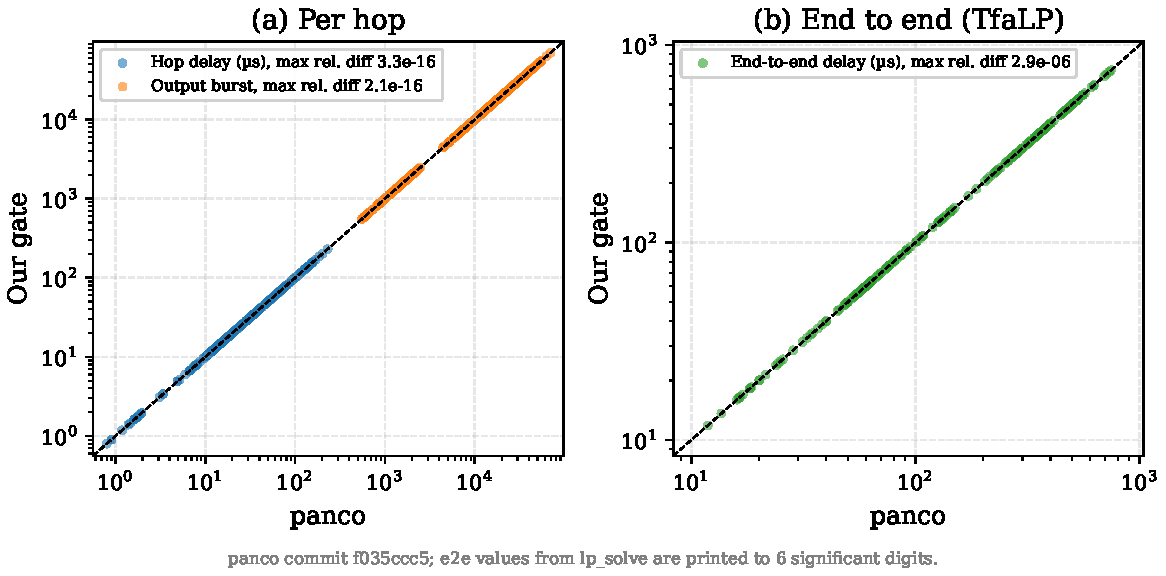
\includegraphics[width=\columnwidth]{panco_agreement.pdf}
        \caption{Bounds of the gate against panco, per hop and end to end.}
        \label{fig:panco}
    \end{figure}

%----------------------------------------------------------

\section{Experiments and Results}
\label{sec:results}

    \subsection{Setup}

        \inlinecode{experiments/benchmark_gate.py} runs, on each topology and for 10 seeds, a greedy proposer that submits 1,000 random requests in arrival order and keeps every accepted flow. Both gates process the same sequence with $C = 1$\,Gbit/s and $t_{proc} = 1\,\mu$s; every admitted set of the incremental gate is then simulated for 10\,ms. Results are written to \inlinecode{results/requests.csv} and \inlinecode{results/simulation.csv}, and \inlinecode{plot_figures.py} draws the figures. All workloads and simulations are seeded; only the timing columns depend on the machine (single-threaded CPython~3.14).

    \subsection{Results}

        \tabref{tab:results} summarises the measurements.

        \begin{table}[H]
            \caption{Results over 10 seeds $\times$ 1,000 requests}
            \label{tab:results}
            \begin{tabular}{
                >{\raggedright\arraybackslash}p{0.40\columnwidth}
                >{\raggedleft\arraybackslash}p{0.21\columnwidth}
                >{\raggedleft\arraybackslash}p{0.21\columnwidth}
            }
            \toprule
            \textbf{Quantity} & \textbf{56 ports} & \textbf{144 ports} \\
            \midrule
            Accepted requests (all) & first 50 & first 200 \\
            Admitted after 1,000 & $150 \pm 14$ & $342 \pm 22$ \\
            Median time, full gate & 3.10\,ms & 7.32\,ms \\
            Median time, incremental & 1.62\,ms & 3.33\,ms \\
            Speed-up of incremental & $1.97\times$ & $2.24\times$ \\
            Ports recomputed (median) & 24 of 56 & 49 of 144 \\
            \bottomrule
            \end{tabular}
            \tabletext{Over all runs both gates give identical verdicts and bit-identical bounds. No simulated delay exceeds its bound over 4,915 admitted flows.}
        \end{table}

        The incremental gate's advantage grows with the network because the affected region becomes a smaller fraction of the ports (\figref{fig:time}). In simulation (\figref{fig:sim}), the median ratio of observed delay to bound is 0.19 for class 0 and 0.10 for class 1, with maxima of 0.71 and 0.43. Admission saturates because TFA is pessimistic (\figref{fig:rate}); class 0 is accepted slightly more often, since its priority shields it from most interference.

        \begin{figure}[H]
            \centering
            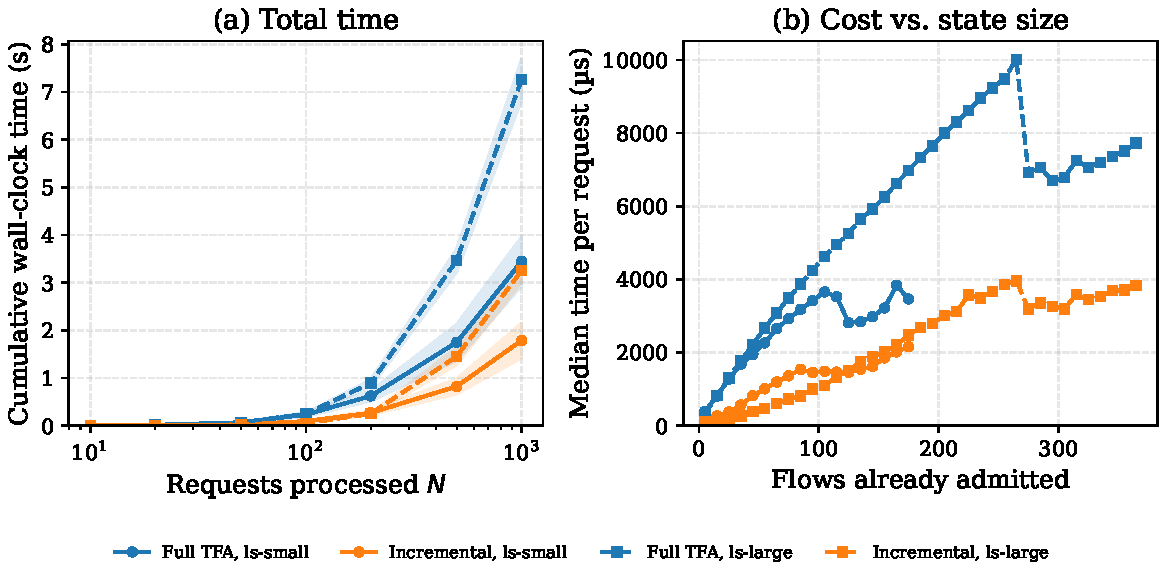
\includegraphics[width=\columnwidth]{scalability.pdf}
            \caption{Run time of the full and incremental gates: (a) cumulative time; (b) median time per request against the number of admitted flows.}
            \label{fig:time}
        \end{figure}

        \begin{figure}[H]
            \centering
            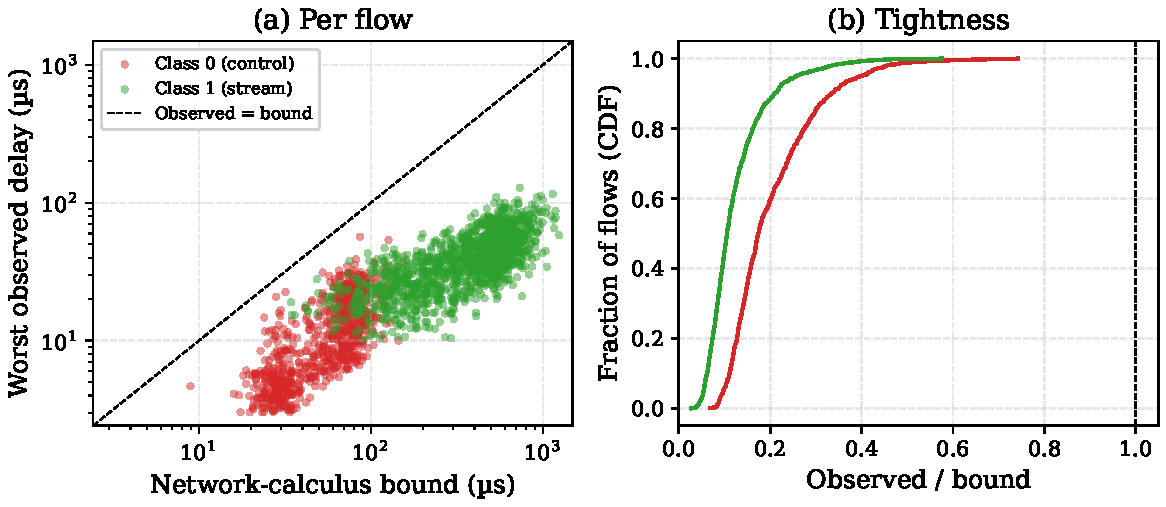
\includegraphics[width=\columnwidth]{bound_tightness.pdf}
            \caption{Worst simulated delay against the bound for 4,915 admitted flows.}
            \label{fig:sim}
        \end{figure}

        \begin{figure}[H]
            \centering
            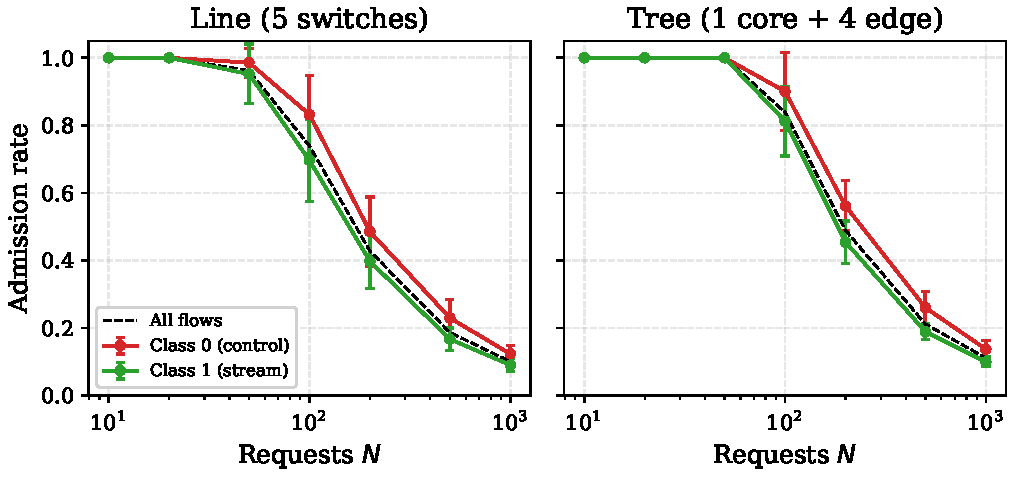
\includegraphics[width=\columnwidth]{admission_rate.pdf}
            \caption{Fraction of the first $N$ requests accepted, per class (mean $\pm$ std over 10 seeds).}
            \label{fig:rate}
        \end{figure}

    \subsection{Tests}

        The 18 unit tests (\inlinecode{python -m pytest -q} in \inlinecode{src/}) cover the hand-computed example to $10^{-12}$, the three rejection cases, full-versus-incremental equality with exact float comparison on both topologies, the locality and validity of incremental certificates, the checker's rejection of a tampered certificate (a halved hop delay, caught by C5; an omitted flow, caught by C0), and the simulator.

%----------------------------------------------------------

\section{Scope and Limits of the Implementation}

    \begin{itemize}
        \item \textbf{Model.} One link rate, fixed shortest-path routing, feed-forward port dependencies and strict NP-SP. Credit-based and time-aware shapers, frame preemption and clock effects are not modelled; Ethernet overheads must be folded into $L_f$, $b_f$ and $r_f$.
        \item \textbf{Analysis.} TFA bounds each port separately. It is sound but pessimistic compared with analyses that pay bursts only once along a path~\cite{bouillard2018dnc}; pessimism lowers the admission rate but never admits an unsafe flow.
        \item \textbf{Arithmetic.} The checker uses floating point with the tolerance \eqref{eq:ge}, which the soundness argument does not account for; exact rational arithmetic would remove this gap.
        \item \textbf{Operations.} Only flow additions are implemented: no removal, no batched changes, and only a greedy proposer.
    \end{itemize}

%----------------------------------------------------------

\section*{Reproduction}
\addcontentsline{toc}{section}{Reproduction}

    All the source code is available at \href{https://github.com/hazel260802/network-calculus}{github.com/hazel260802/network-calculus}. From the \inlinecode{src} directory, run:
    \begin{itemize}
        \item \inlinecode{pip install -r requirements.txt}
        \item \inlinecode{python -m pytest -q}
        \item \inlinecode{python experiments/benchmark_gate.py}
        \item \inlinecode{python experiments/plot_figures.py}
    \end{itemize}
    The panco check needs panco at commit \inlinecode{f035ccc5}, set as \inlinecode{PANCO_PATH}, and lp\_solve for the end-to-end mode:
    \begin{itemize}
        \item \inlinecode{python validation/panco_check.py --mode hop}
        \item \inlinecode{python validation/panco_check.py --mode e2e}
    \end{itemize}

%----------------------------------------------------------

\printbibliography

\end{document}
